% !TeX program = pdflatex
\documentclass[11pt]{article}

% ---------- Fonts & Layout ----------
\usepackage[T1]{fontenc}
\usepackage{lmodern}
\usepackage[margin=1in]{geometry}
\usepackage{microtype}
\usepackage[dvipsnames]{xcolor}
\usepackage{fancyhdr}
\pagestyle{fancy}
\lhead{LaTeX Showcase}
\rhead{\today}
\cfoot{\thepage}

% ---------- Math & Symbols ----------
\usepackage{amsmath, amssymb, amsthm, mathtools}
\usepackage{siunitx}
\sisetup{output-exponent-marker=\text{e}, group-minimum-digits=4}
\usepackage{physics}

% ---------- Figures, Tables, Code ----------
\usepackage{graphicx}
\usepackage{subcaption}
\usepackage{booktabs}
% Add enumitem for customized list spacing/labels (fixes itemize option errors)
\usepackage{enumitem}
\usepackage{tikz}
\usepackage{pgfplots}
\pgfplotsset{compat=1.18}
\usepackage{listings}
\lstset{language=Python, basicstyle=\ttfamily\small, frame=single, breaklines=true,
  numbers=left, numberstyle=\tiny, numbersep=5pt, columns=fullflexible}
\usepackage{tcolorbox}
\tcbuselibrary{skins, breakable}
\usepackage{algorithm}
\usepackage{algpseudocode}

% ---------- Hyperlinks & Clever References ----------
\usepackage[colorlinks=true,linkcolor=MidnightBlue,citecolor=MidnightBlue,urlcolor=MidnightBlue]{hyperref}
\usepackage[nameinlink,noabbrev]{cleveref}

% ---------- Theorems & Macros ----------
\newtheorem{theorem}{Theorem}
\newtheorem{definition}{Definition}
\newcommand{\R}{\mathbb{R}}
\newcommand{\vect}[1]{\boldsymbol{#1}}

\title{A Two-Page LaTeX Showcase\\\large Formatting, Math, Figures, Tables, Algorithms, and More}
\author{Your Name}
\date{\today}

\begin{document}
\maketitle
\begin{abstract}
This compact document demonstrates a broad range of \LaTeX{} features: typography and structure; inline and display mathematics with references; theorem environments; figures (including a TikZ diagram and a plotted function); professional tables; code listings; boxed callouts; and a short algorithm. Hyperlinks and clever cross-references are also showcased.
\end{abstract}

\section{Typography \\ \& Structure}
\LaTeX{} excels at beautiful typography. You get automatic hyphenation, ligatures, and kerning out of the box. You can emphasize text (\emph{emphasis}), make it \textbf{bold}, or use \textsc{Small Caps}. You can add footnotes\footnote{This is a footnote demonstrating automatic numbering and layout.} and hyperlinks (e.g., to the \href{https://www.latex-project.org}{\LaTeX{} Project}). Lists are easy to customize:
% Customized itemize list; requires enumitem
\begin{itemize}[leftmargin=1.5em]
  \item Compact bullet list with custom margins.
  \item Numbered lists work similarly:
    \begin{enumerate}[label=\arabic*.]
      \item First item
      \item Second item
    \end{enumerate}
\end{itemize}
\begin{tcolorbox}[title=Callout: Why \LaTeX?,colback=blue!3!white,colframe=MidnightBlue,enhanced,breakable]
\LaTeX{} separates content from presentation, giving you consistent, high-quality typesetting and flexible cross-referencing, bibliographies, and math.
\end{tcolorbox}

\section{Mathematics}
Inline math $e^{i\pi}+1=0$ sits nicely in text; display math centers and numbers equations. For example, the Gaussian integral in \cref{eq:gauss} and Euler's identity in \cref{eq:euler}:
\begin{equation}\label{eq:gauss}
\int_{-\infty}^{\infty} e^{-x^2}\,dx = \sqrt{\pi}.
\end{equation}
\begin{align}
  e^{i\pi} + 1 &= 0, \label{eq:euler}\\
  \nabla f(\vect{x}) &= \begin{bmatrix} \partial f/\partial x_1 & \cdots & \partial f/\partial x_n \end{bmatrix}^{\!\top}.
\end{align}
Piecewise definitions, matrices, and units are straightforward:
\[
  f(x) = \begin{cases}
    x^2, & x \ge 0, \\
    -x,  & x < 0,
  \end{cases}\qquad
  A = \begin{bmatrix}1 & 2 \\ 3 & 4\end{bmatrix},\qquad v=\SI{3.0e8}{\meter\per\second}.
\]

\begin{theorem}[Cauchy--Schwarz]
For any vectors $u,v\in\R^n$, $\,|\langle u,v\rangle|\le \|u\|\,\|v\|$.
\end{theorem}
\begin{proof}
Consider $g(t)=\|u-t v\|^2\ge 0$. Expanding and minimizing the quadratic in $t$ yields $\langle u,v\rangle^2\le \|u\|^2\,\|v\|^2$.
\end{proof}

\section{Figures and Plots}
\Cref{fig:diagram,fig:plot} show a vector diagram (TikZ) and a plotted function (PGFPlots) side by side.
\begin{figure}[h]
  \centering
  \begin{subfigure}{.48\textwidth}
    \centering
    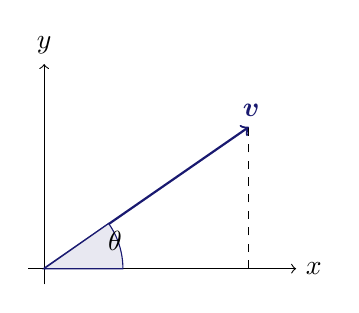
\begin{tikzpicture}[scale=1]
      \draw[->] (-0.2,0) -- (3.2,0) node[right]{$x$};
      \draw[->] (0,-0.2) -- (0,2.6) node[above]{$y$};
      \draw[thick,->,MidnightBlue] (0,0) -- (2.6,1.8) node[above]{$\,\vect v$};
      \draw[dashed] (2.6,0) -- (2.6,1.8);
      \filldraw[fill=MidnightBlue!10,draw=MidnightBlue] (0,0) -- (1,0) arc(0:35:1) -- cycle;
      \node at (0.9,0.35){$\theta$};
    \end{tikzpicture}
    \caption{A simple TikZ diagram.}
    \label{fig:diagram}
  \end{subfigure}\hfill
  \begin{subfigure}{.48\textwidth}
    \centering
    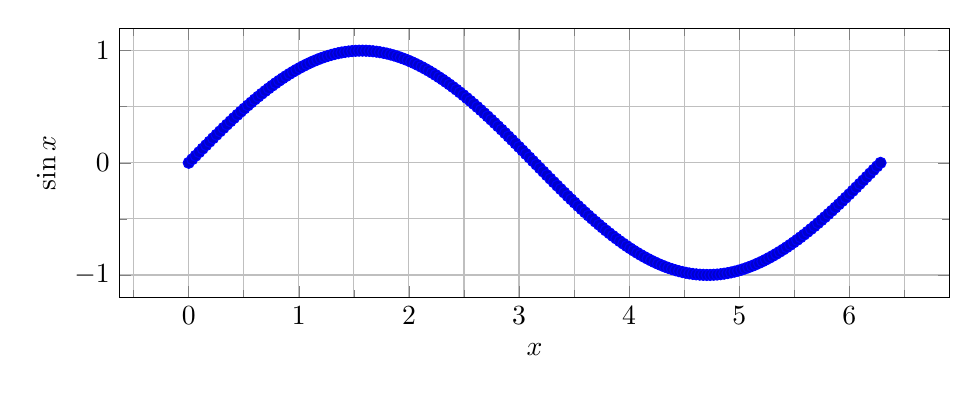
\begin{tikzpicture}
      \begin{axis}[
        xlabel={$x$}, ylabel={$\sin x$},
        width=\linewidth, height=5cm,
        grid=both, minor tick num=1,
      ]
        \addplot+[domain=0:6.283, samples=200] {sin(deg(x))};
      \end{axis}
    \end{tikzpicture}
    \caption{A plot via PGFPlots.}
    \label{fig:plot}
  \end{subfigure}
  \caption{Graphics generated directly in \LaTeX{}.}
\end{figure}

\section{Tables}
\Cref{tab:results} demonstrates professional tables with \texttt{booktabs} and aligned numbers via \texttt{siunitx}.
\begin{table}[h]
  \centering
  \begin{tabular}{l S[table-format=2.2] S[table-format=1.3]}
    \toprule
    Method & {Accuracy (\%)} & {Loss} \\
    \midrule
    Baseline & 74.25 & 0.812 \\
    Improved & 82.10 & 0.523 \\
    FancyNet & 88.03 & 0.401 \\
    \bottomrule
  \end{tabular}
  \caption{Aligned numeric columns with \texttt{siunitx}.}
  \label{tab:results}
\end{table}

\section{Code Listings}
\Cref{lst:python} shows a Python snippet with line numbers and automatic wrapping.
\begin{lstlisting}[caption={Tiny gradient descent in Python.},label={lst:python}]
import math

# Objective: f(x) = (x-3)^2
x, lr = 10.0, 0.1
for step in range(50):
    grad = 2 * (x - 3)
    x -= lr * grad
print(f"Converged to {x:.4f}")
\end{lstlisting}

\section{Algorithms}
Pseudocode with the \texttt{algorithmicx} package (\cref{alg:euclid}):
\begin{algorithm}[h]
  \caption{Euclidean GCD}\label{alg:euclid}
  \begin{algorithmic}[1]
    \Procedure{GCD}{$a,b$}
      \While{$b \ne 0$}
        \State $(a,b) \gets (b,\, a \bmod b)$
      \EndWhile
      \State \Return $a$
    \EndProcedure
  \end{algorithmic}
\end{algorithm}

\section{Citations}
You can include citations and a bibliography. Here we use a simple manual list; for larger projects, consider \texttt{biblatex}.

\begin{thebibliography}{9}
\bibitem{lamport} Leslie Lamport. \emph{\LaTeX: A Document Preparation System}. Addison--Wesley, 2nd ed., 1994.
\bibitem{knuth} Donald E. Knuth. \emph{The \TeX book}. Addison--Wesley, 1984.
\end{thebibliography}

\end{document}
